\documentclass[tikz,border=4pt]{standalone}
\usepackage{pgfplots}
\usepgfplotslibrary{groupplots}
\pgfplotsset{compat=1.18}
\begin{document}
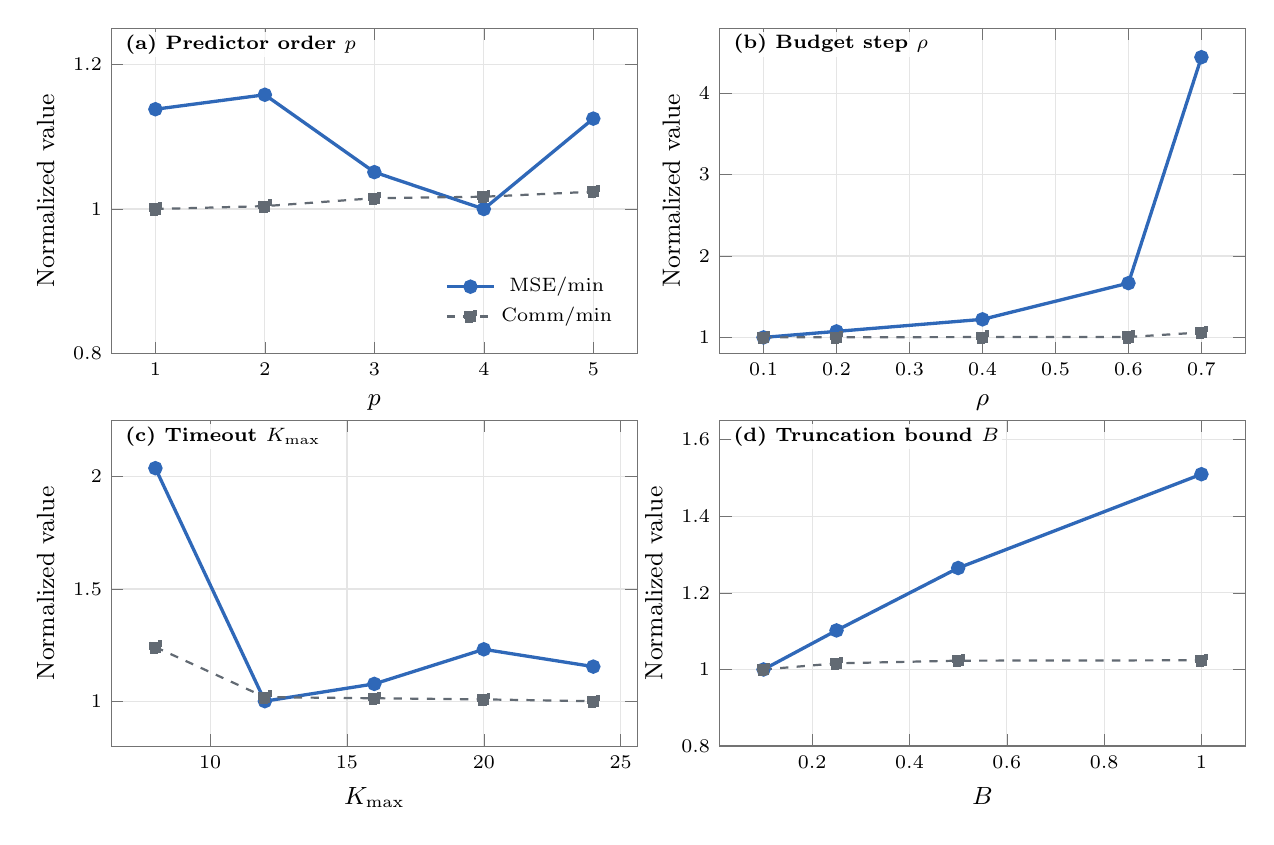
\begin{tikzpicture}
\definecolor{EBlue}{HTML}{2F68B8}
\definecolor{ENeutral}{HTML}{626A73}
\begin{groupplot}[
  group style={group size=2 by 2, horizontal sep=1.05cm, vertical sep=0.85cm},
  width=3.25in,
  height=2.25in,
  tick label style={font=\scriptsize},
  label style={font=\small},
  title style={font=\scriptsize\bfseries, at={(0.02,0.94)}, anchor=north west, fill=white, fill opacity=0.88, text opacity=1, inner sep=1pt},
  grid=major,
  major grid style={draw=black!10},
  axis line style={black!55},
  tick style={black!55},
  ylabel={Normalized value},
  ymin=0.8,
]
\nextgroupplot[title={(a) Predictor order $p$}, xlabel={$p$}, ymax=1.25, legend style={font=\scriptsize, draw=none, fill=none, at={(0.98,0.05)}, anchor=south east}]
  \addplot[mark=*, very thick, color=EBlue, mark options={fill=EBlue, draw=EBlue}] coordinates {(1,1.138) (2,1.158) (3,1.051) (4,1.000) (5,1.125)};
  \addlegendentry{MSE/min}
  \addplot[mark=square*, thick, dashed, color=ENeutral, mark options={fill=ENeutral, draw=ENeutral}] coordinates {(1,1.000) (2,1.004) (3,1.015) (4,1.017) (5,1.024)};
  \addlegendentry{Comm/min}
\nextgroupplot[title={(b) Budget step $\rho$}, xlabel={$\rho$}, ymax=4.8]
  \addplot[mark=*, very thick, color=EBlue, mark options={fill=EBlue, draw=EBlue}] coordinates {(0.1,1.000) (0.2,1.074) (0.4,1.222) (0.6,1.667) (0.7,4.444)};
  \addplot[mark=square*, thick, dashed, color=ENeutral, mark options={fill=ENeutral, draw=ENeutral}] coordinates {(0.1,1.000) (0.2,1.002) (0.4,1.004) (0.6,1.005) (0.7,1.061)};
\nextgroupplot[title={(c) Timeout $K_{\max}$}, xlabel={$K_{\max}$}, ymax=2.25]
  \addplot[mark=*, very thick, color=EBlue, mark options={fill=EBlue, draw=EBlue}] coordinates {(8,2.038) (12,1.000) (16,1.077) (20,1.231) (24,1.154)};
  \addplot[mark=square*, thick, dashed, color=ENeutral, mark options={fill=ENeutral, draw=ENeutral}] coordinates {(8,1.241) (12,1.018) (16,1.013) (20,1.008) (24,1.000)};
\nextgroupplot[title={(d) Truncation bound $B$}, xlabel={$B$}, ymax=1.65]
  \addplot[mark=*, very thick, color=EBlue, mark options={fill=EBlue, draw=EBlue}] coordinates {(0.10,1.000) (0.25,1.102) (0.50,1.265) (1.00,1.510)};
  \addplot[mark=square*, thick, dashed, color=ENeutral, mark options={fill=ENeutral, draw=ENeutral}] coordinates {(0.10,1.000) (0.25,1.016) (0.50,1.023) (1.00,1.024)};
\end{groupplot}
\end{tikzpicture}
\end{document}
